\documentclass[12pt]{article}
\usepackage[utf8]{inputenc}
\usepackage[a4paper, total={6in,4in}]{geometry}
\usepackage{geometry}
\usepackage{amsmath}
\usepackage{amssymb}
\usepackage{amsthm}
\usepackage{graphicx}
\usepackage{float}
\usepackage[normalem]{ulem}
\geometry{left=2cm, right=2cm, top=2cm, bottom=2cm}
\newtheorem{manualtheoreminner}{Theorem}
\newenvironment{theorem}[1]{%
  \renewcommand\themanualtheoreminner{#1}%
  \manualtheoreminner
}{\endmanualtheoreminner}
\newtheorem*{corollary}{Corollary}
\newtheorem*{lemma}{Lemma}
\newtheorem{example}{Example}
\newtheorem{definition}{Definition}
\newtheorem*{remark}{Remark}
\newtheorem{solution}{Solution}
\newenvironment{pro}{\begin{proof}}{\end{proof}}

\graphicspath{{./img/}}
\makeatletter
\newenvironment{usecounterof}[2]{%
  \def\@tempb{#1}%
  \expandafter\renewcommand\csname the#1\endcsname{\ref{#2}}\@nameuse\@tempb}{%
    \@nameuse{end\@tempb}\addtocounter\@tempb{-1}}
\makeatother



\begin{document}

\textbf{Planarity}

\textbf{Problem:} Let $G$ be a graph. Can $G$ be drawn in such a manner so that no two edges intersect?


\begin{example}

	Any drawing of $K_{5}$ or $K_{3,3}$ have (at lease) 2 edges which cross (Proof to come)
	\begin{center}
		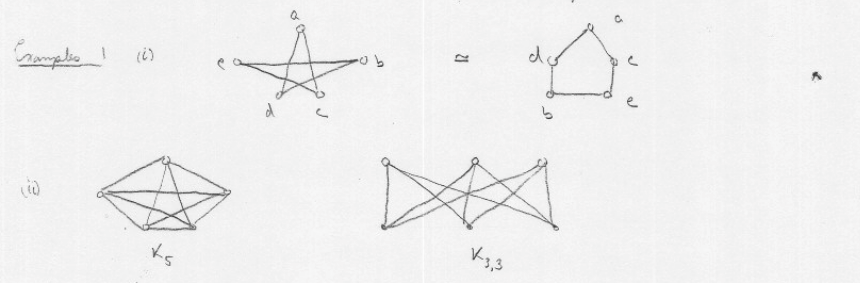
\includegraphics[width=15cm,height=7cm]{example1}
	\end{center}
\end{example}


\begin{definition}
	A graph $G$ is said to be planer if it can be drawn in $\mathbb{R}^{2}$ so that no two edges cross. Such a drawing is called a plane drawing. The graph associated with a plane drawing is usually refered to as a plane graph.
\end{definition}

\begin{remark}

	\begin{enumerate}
		\item Any subgraph of a planer graph is planer.
		\item Every plane graph is planar.


		      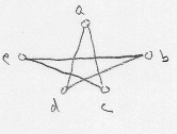
\includegraphics[width=3cm, height=2cm]{notplane}
		      is a planer but not plane.
	\end{enumerate}

\end{remark}


Our aim is to determine condition which ensures that a graph $G$ is planar. Let $G$ be a plane graph. Consider the set $S$ obtained from $\mathbb{R}^{2}$ by deleting (the vertices and edges) of $G$.
We observe that $S$ is the disjoint union of finitely many subsets $F_{1}, F_{2},\dots F_{l}$ of $\mathbb{R}^{2}$ having the following two properties:

\begin{enumerate}
	\item Any two points of $F_{i}$ can be joined by a curve not crossing $G$.
	\item Any curve in $\mathbb{R}^{2}$ which joins a point of $F_{i}$ to one of $F_{j}, i\neq j, $ \underline{must} cross $G$
\end{enumerate}


\begin{definition}
	Let $G$ be a plane graph. The sets $F_{1}, \dots F_{l}$ described above are called the \underline{faces} of $G$.
\end{definition}

\begin{example}\label{a-thm}
	Faces

	\begin{center}
		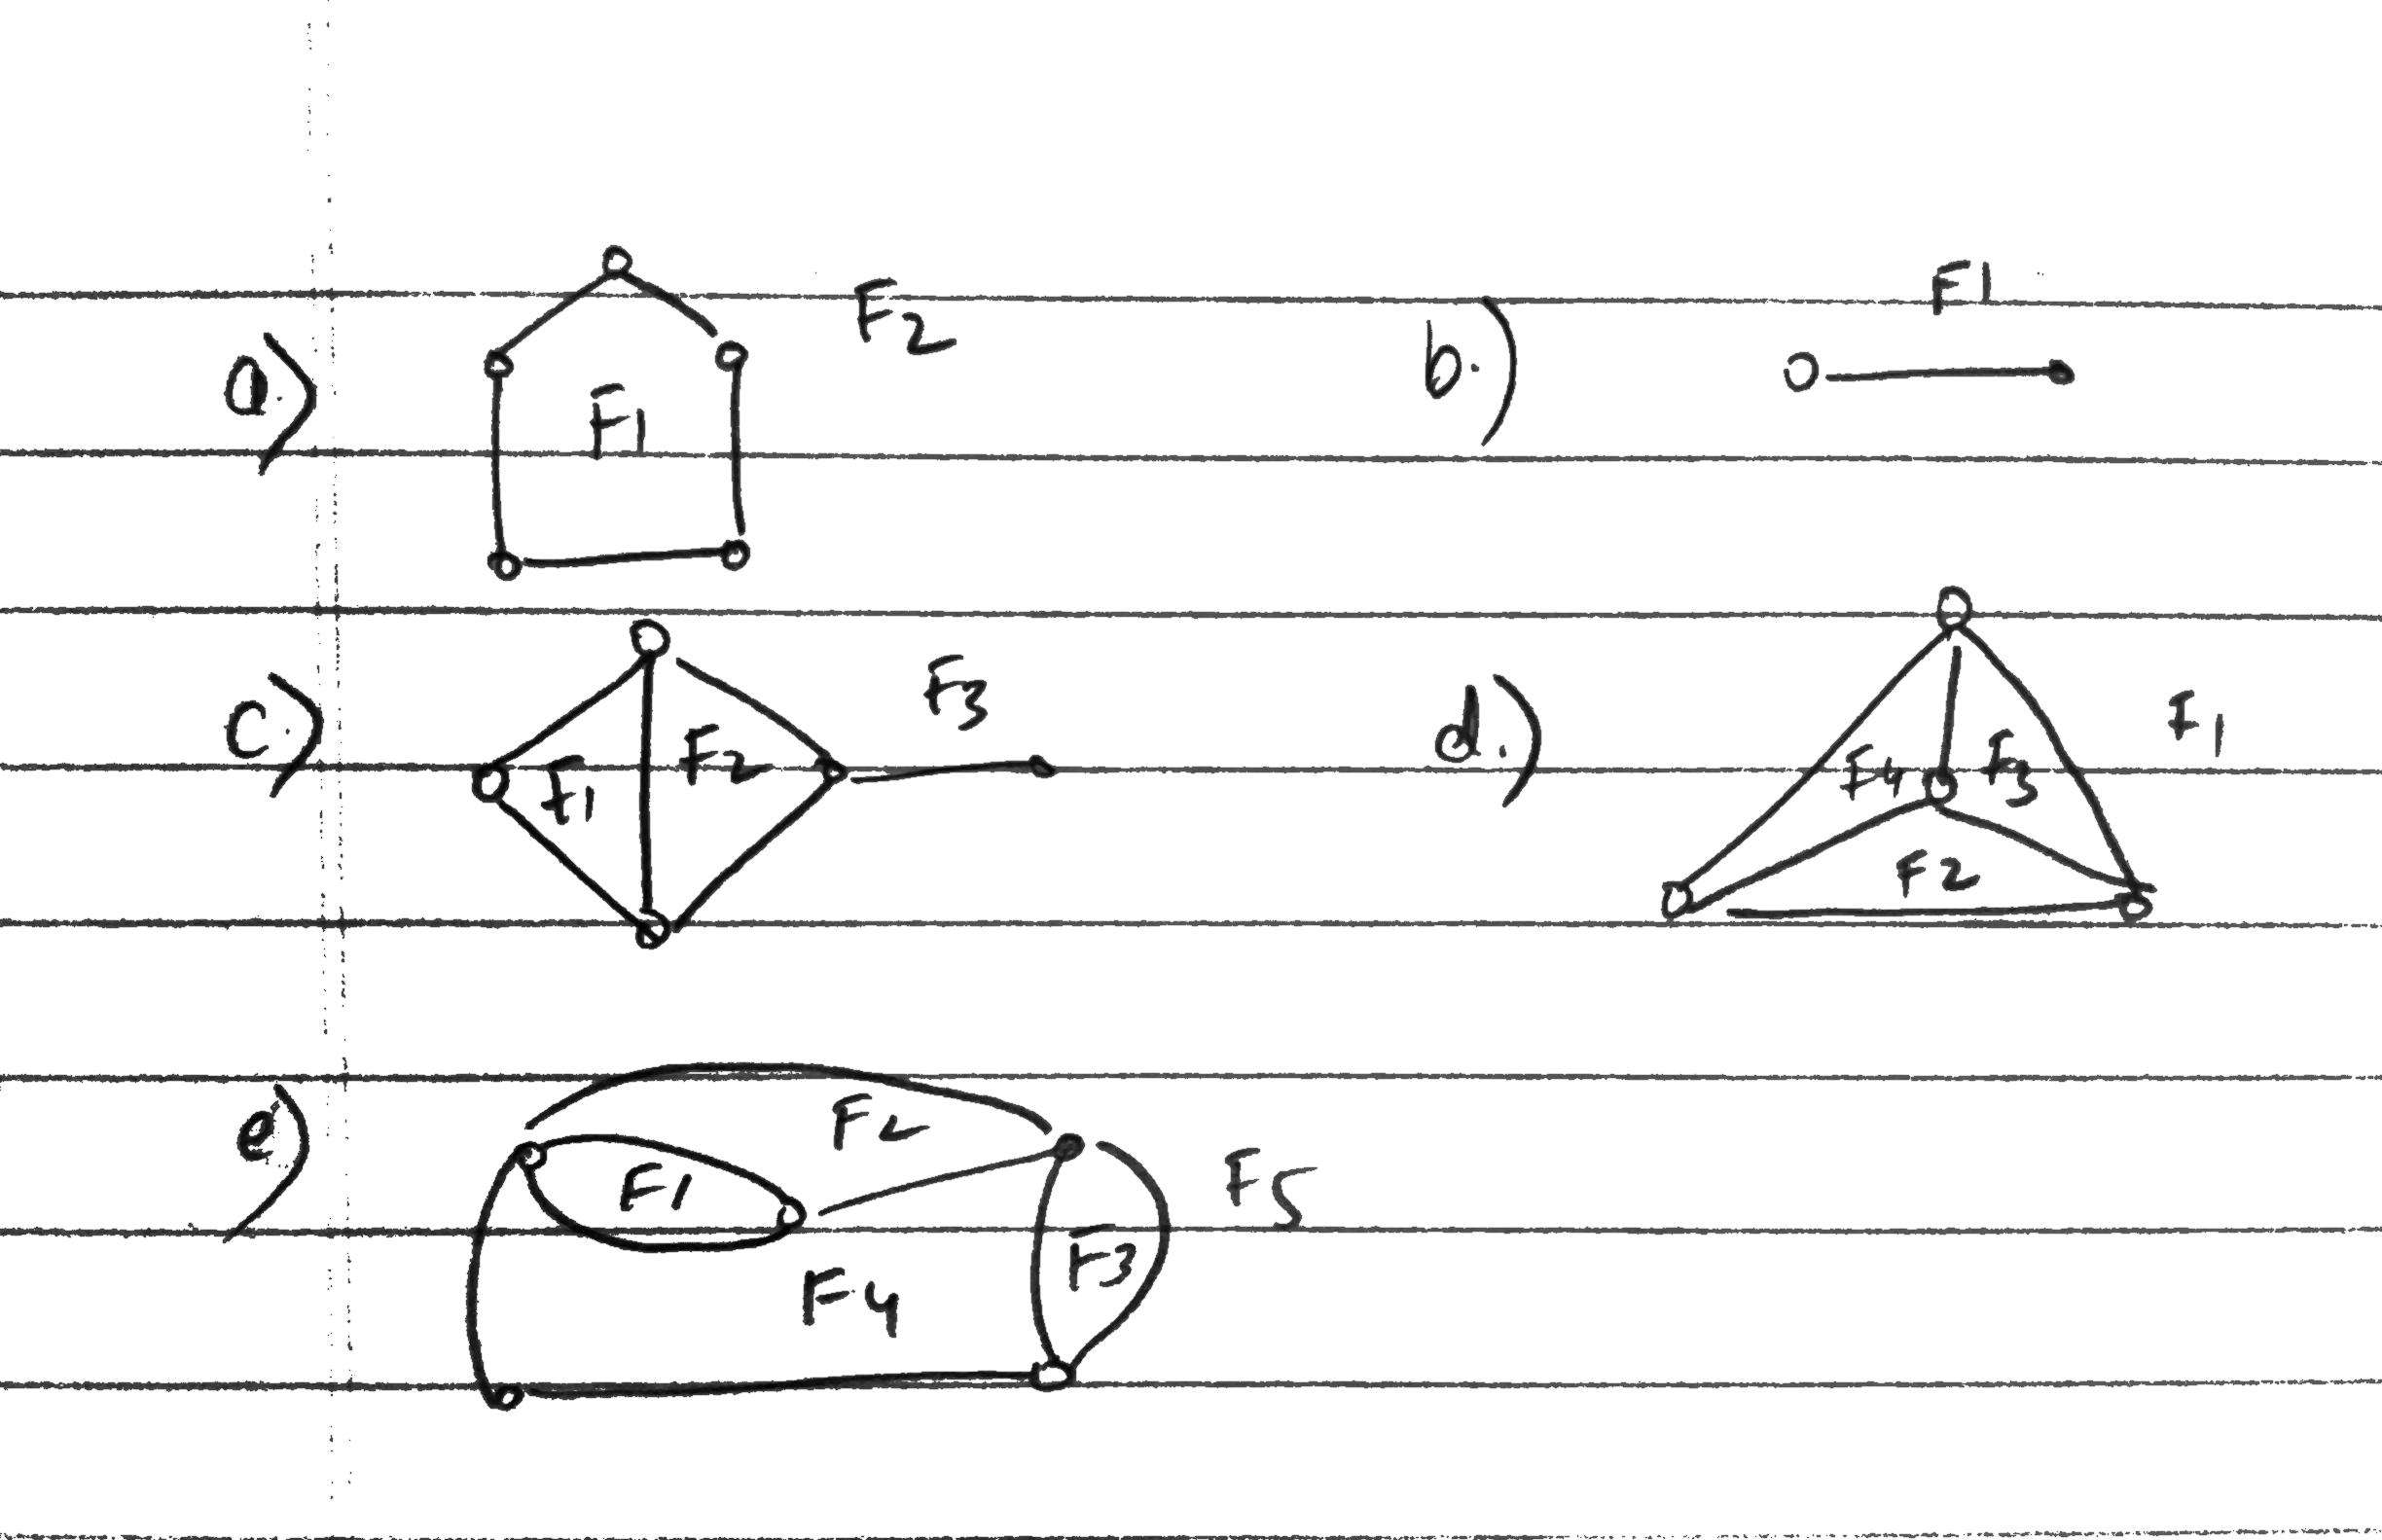
\includegraphics[width=12cm, height=7cm]{example2}
	\end{center}

\end{example}

\begin{remark}
	One face is always unbounded, with the remaining faces all bounded.
\end{remark}


\begin{definition}
	Let $F$ be a face of a plane graph $G$. The boundary of $F$ consists of a finite \# of vertices and edges of $G$

	The length of a closed walk around the boundary of $F$ is called the \underline{degree of $F$}, usually denoted $\deg F$

\end{definition}


\begin{usecounterof}{example}{a-thm} (Cont.)
	\begin{enumerate}
		\item $\deg F_{1} = \deg F_{2} = 5$
		\item $\deg F_{2} = 2$ the closed walk is $x\to y \to x$
		\item $\deg F_{1} = \deg F_{2} = 3$\\
		      $\deg F_{3} = 6$
	\end{enumerate}


\end{usecounterof}


\begin{theorem}{1}
	\textit{(Euler's Formula, 1780)} Let $G$ be a connected plane graph. If $G$ has $n$ nodes and $f$ faces then

	\[n - m + f = 2\]
	proof of \textbf{Theorem 1} requires a couple of preliminarily lemmas.
\end{theorem}

\begin{lemma}
	Let $G$ be a plane graph. $G$ contains a cycle if and only if the number of faces of $G \ge 2$.
\end{lemma}

\begin{pro}
	$\rightarrow$ Let $C$ be a cycle of $G$. Let $x$ and $y$ be in the interior and exterior of $C$, respectively, then any curve in $\mathbb{R}^{2}$ connecting $x$ and $y$ must cross $C$, have cross $G$

	\begin{center}
		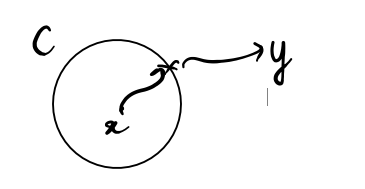
\includegraphics[width=7cm,height=4cm]{circle_proof}
	\end{center}

	Choosing $x, y$ not lying on $G$ $x$ and $y$ belong to different faces of $G$.

	$\leftarrow$ The absence of a cycle, $G$ is a forest. On induction on the number of components of $G$ shows $G$ has only one (unbounded) face.

	\begin{center}
		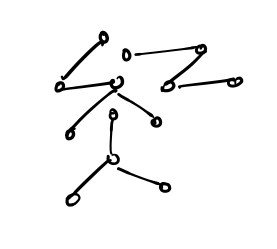
\includegraphics[width=7cm,height=4cm]{circle_proof2}
	\end{center}

\end{pro}



\begin{lemma}
	Let $e$ be an edge of a plane graph $G$.
	\begin{enumerate}
		\item If $e$ is a bridge then it lies on boundary of exactly one face.
		\item if $e$ is not a bridge then it lies on the boundary of exactly two faces of $G$
	\end{enumerate}
\end{lemma}


\begin{pro}
	\begin{enumerate}
		\item Let $H_{1}$ and $H_{2}$ be the components of $G\textbackslash e$. The edge $e$ lies in face $F_{1}$ of $H_{1}$, as well as a face $F_{2}$ of $H_{2}$.
		      The intersetion $F_{1}\cap F_{2}$ contains a unique face $F_{o}$ of $G$. $e$ lies on the boundary of $F_{o}$ and is the unique face of $G$.
		      \begin{center}
			      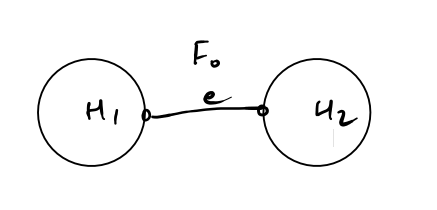
\includegraphics[width=7cm, height=4cm]{proof2}
		      \end{center}

		\item Let $C$ be a cycle containing $e$. The edge $e$ lies on the boundary of one face lying in the interior of $C$ and one face lying in the exterior of $C$.
		      Thus, $e$ lies on the boundary of at least $2$ faces of $G$.

		      \begin{center}
			      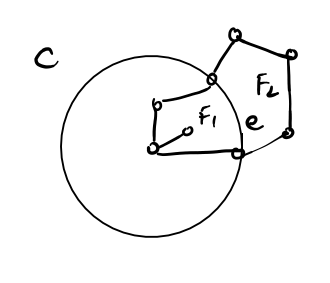
\includegraphics[width=7cm, height=5cm]{proof2.1}
		      \end{center}


		      The fact faces are disjoint can be used to show that $e$ lies on the boundary of at most $1$ face lying in the interor of $C$, and one face lying in the exterior of $C$. THen $e$ lies in the boundary of at most 2 faces.

	\end{enumerate}

\end{pro}



\begin{corollary}

	(Handshaking Lemma for Planar Graphs)
	If $G$ is a plane graph of size $m$ then

	\[2m = \Sigma_{\text{faces } F} \deg  F\]
\end{corollary}

\begin{pro}
	Each edge $e$ of $G$ contributes 2 to the sum on the right:

	If $e$ is a bridge lying on the face $F_{o}$ then it contributes 2 to $\deg F_{o}$ and 0 to the remaining $\deg F$.


	If $e$ is not a bridge then it contributes 1 to the degree of two distinct faces of $G$, and 0 to the remaining.
\end{pro}


\begin{pro}

	Proof of Euler's Formula

	We proved by induction on $\#$ of faces of $G$ on the case $f=1$. \textbf{Lemma 2} asserts $G$ is a forest, where $G$ is a tree.
	Thus, $m=n-1$, and hence $n-m +f = n-(n-1)+1 = 2$

	Assume the result is true $f$ connected plane graph $H$ having $f$ faces, and let $G$ have $f+1$ faces, say $F_{1}, F_{2}, \dots, F_{l}, F_{l+1}$.
	If $n = \vert G\vert, m = e(G)$ then we are required to show

	\[n-m +(f+1) = 2\]

	Since $f+1\ge 2$, $G$ contains a cycle $C$ (\textbf{Lemma 2}). Fix an edge $e$ lying on $C$. Assume $e$ is not a bridge of $G$. \textbf{Lemma 2} ensures that $e$ lies on the boundary of 2 distince faces of $G$, say $F_{l}$ and $F_{l+1}$.
	\begin{center}
		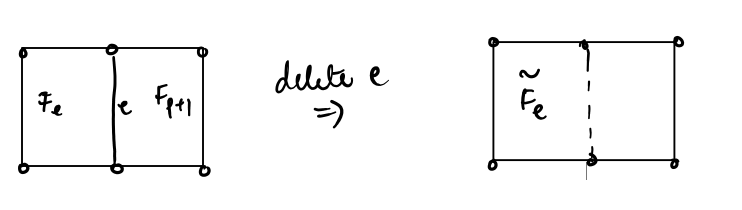
\includegraphics[scale=0.5]{eulerproof}
	\end{center}


	Construst the subgraph $H=G\textbackslash e$. We note $H$ is a connected plane graph of order $n$ and size $m-1$.
	Furthermore, the number of faces of $H$ is $f$. denoted each of the faces $F_{1}, f_{2},\dots F_{l-1}$ of $G$ occur on faces of $H$. Assume $e$ does not appear in the boundary of any of these faces.

	Teh remaining faces of $H$ is obtained by joining $F_{l}$ and $F_{l+1}$ along the edge $e$.

	\[\hat{F_{l}} = F_{l} \cup F_{l+1} \cup e\]

	Since $H$ has $f$ faces, the indcuntion hypotheses allows in $G$ to conclude that

	\[ 2 = n- (m-1) + f = n - m + (f+1)\]
	as required

\end{pro}


\begin{corollary}

	Let $G$ be a connected planer graph. Each plane drawing of $G$ has the same number of faces, namely $2+m - n$

	Euler's formula can be used to obtain a necessary condition for a simple connected graph to be planar.
\end{corollary}

\begin{definition}
	Let $G$ be a graph, If $G$ contains a cycle then the \textbf{girth} $gr(G)$ is defined as the length of the smallest cycle in $G$. If $G$ is a forest then we set $gr(G) = \infty$
\end{definition}

\begin{example}
	Girth
	\begin{center}
		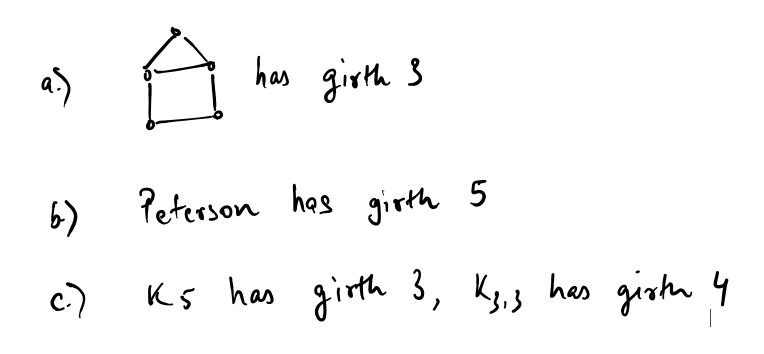
\includegraphics[scale=0.5]{example}
	\end{center}
\end{example}


\begin{remark}
	If $G$ is simple then $gr(G) \ge 3$
\end{remark}


\begin{theorem}{4}
	Let $G$ be a connected simple planar graph. If $G$ has order $n$ and size $m$ then

	\begin{align} m \le \begin{cases} n-1                          & \text{if } gr(G) = \infty             \\
              \frac{gr(G)}{gr(G) - 2}(n-2) & \text{ if  } gr(G) \text{ is finite }\end{cases}
	\end{align}
\end{theorem}


\begin{pro}
	If $gr(G) = \infty$ then $G$ is a tree, hence $m = n-1$ if $gr(G)$ is finite then $G$ has $\ge 2$ faces. In this case, the boundary of each face of $G$ contains a cycle, hence
	\[\deg (F) \ge gr(G)\]

	If each face $F$ of $G$. therfore, if $f = \#$ of faces of $G$ then the handshaking lemma of planer graphs

	\[ 2m = \Sigma_{\text{faces} F} \deg F \ge \Sigma gr(G) = gr(G) f\]

	From Euler's formula, $f = 2+m-n$, substitues $f_{i}$ in the preceding yields

	\[2m \ge gr(G) (2+m-n)\]
\end{pro}


\begin{example}

	\begin{enumerate}


		\item  Does there exist a simple connected planar graph $G$ of order 12 and size 40?
		      \begin{solution}

			      Suppose such a graph $G$ exists, Note that $G$ cannot be a tree, hence  $gr(G)$ is finite. Thus, \textbf{Theorem 3} asserts
			      \[40 \ge \frac{gr(G)}{gr(G) - 2} (12 - 2)\]

			      Solving for $gr(G)$
			      \[gr(G) \le \frac{8}{3} < 3\]
			      This contradicts that $gr(G) \ge 3$ No such $G$ exists.
		      \end{solution}

		\item Let $G$ be a planar graph of size  and girth 5. What can one  say about $n = \vert G\vert$

		      \begin{solution}
			      From \textbf{Theorem 2}
			      \[14 \le \frac{5}{5-2} (n-2)\]
			      solving $f$ n yields $n\ge 52/5$ some $n$ is an integer $n\ge 11$.
		      \end{solution}
	\end{enumerate}
\end{example}


\begin{corollary}
	$K_{5}$ and $K_{3,3}$ are non-planar
\end{corollary}


\textbf{Proof here}


\textbf{Exercise Show that Peterson is non-planar}


\begin{corollary}
	Let $G$ be a simple connected planar graph.
	\begin{enumerate}
		\item if $G$ has order $n\ge 3$ then $e(G) \le 3n - 6$
		\item Furthermore, if $G$ contains no triangles then $e(G) \le 2n - 4$
	\end{enumerate}

\end{corollary}

\textbf{proof here}


\begin{remark}
	The preceding two results are often used as tools for non-planarity, they are weakter then the full theorem 4.
\end{remark}


\begin{corollary}
	Every simple planar graph $G$ contains a vertex of degree at most $5 (\delta(G) \le 5)$
\end{corollary}

\textbf{proof here}



\begin{example}
	$K_{n}$ is non-planar of $n\ge 7$. Each vertex of $K_{n}$ has degree $n-1 \ge 6$
\end{example}

\begin{example}
	The condition of theorem 4 (as well as it corollories) is only necessary for planarity, not sufficient. For example, the following graph $G$ is non-planar, as it contains a copy of $K_{3,3}$

	\begin{center}
		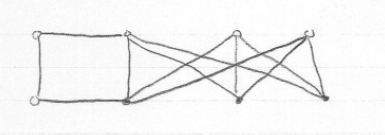
\includegraphics[scale=0.5]{k3_non_planar}
	\end{center}

	On the other hand, $\vert G\vert =8, e(G) = 12 \text{ and } gr(G) = 4$
	\[\frac{4}{4-2} (8-2) = 12\]
\end{example}

\begin{remark}
	Euler's formula can be extended to disconnected plane graphs using induction on the $\#$ of components. If $G$ is aplnar graph of order $n$ size $m$ with $f$ faces and $k$ components then
	\[n- m + f = k +1\]

	There are also analogue for Theorem 3 and its corollories.

	We have already observed that Theorem 3 and its corollories present many necessary conditions for a graph to be planar.

\end{remark}


\begin{definition}
	Let $G$ and $H$ be graphs. $H$ is said to be a \underline{subdivion} of $G$ if the formal graph can be constructed from the latter by introduction a finite \# of new vertices along existing edges.
\end{definition}

\begin{example}

	\begin{center}
		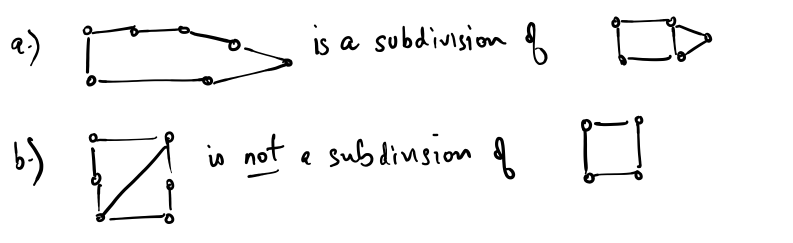
\includegraphics[scale=0.5]{example6}
	\end{center}
	\textbf{c.)} Each cycle graph $C_{n}$ is a subdivision of $C_{1}. C_{n}$ can be obtained from $C_{1}$ by the addition of $n-1$ new vertices on the single edge of $C_{1}$
	\begin{center}
		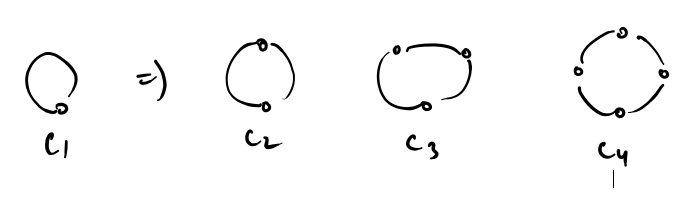
\includegraphics[scale=0.5]{c1graph}
	\end{center}

\end{example}


\begin{remark}
	\begin{enumerate}
		\item The process of subdivion only introduces new vertices of degree 2
		\item Note that if $H$ is a subdivion of $G$ then $H$ has the same shape as $G$.
	\end{enumerate}
\end{remark}

\begin{definition}
	Two graphs $G$ and $H$ are said to be homeomorphism if they are both subdivision of a common graph.
\end{definition}

\begin{example}
	\begin{enumerate}
		\item If $n,m \ge 1$ then $C_{n}$ is homeomorphism to $C_{m}$ as both are subdivion of $C_{1}$.
		\item If $n,m\ge 2$ then $P_{n}$ and $P_{m}$ are homoeomorphism as both are subdivion of $P_{2}$
	\end{enumerate}
\end{example}


\begin{remark}

	\begin{enumerate}
		\item $G$ and $H$ are homeomorphic if the latter can be obtained from the former by a finite sequence of following 2 operations:
		      \begin{enumerate}
			      \item addition of new vertex along an existing edge.
			      \item filling in of an existing verted of degree 2.
		      \end{enumerate}

		      \begin{center}
			      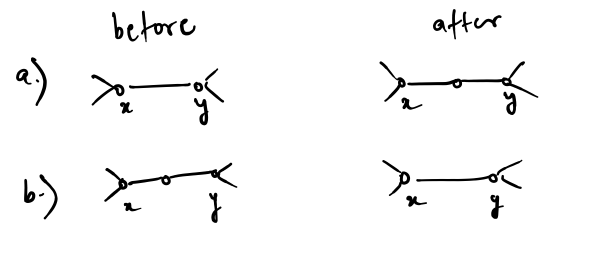
\includegraphics[scale=0.5]{remarkgraph}
		      \end{center}
		\item homeomorphic graphs have the same shape.
	\end{enumerate}
\end{remark}



\begin{theorem}{5}
	A graph is planar if and only if it contains no subgraph homeomorphic to $K_{5}$ or $K_{3,3}$.
\end{theorem}


\begin{example}
	The graph
	\begin{center}
		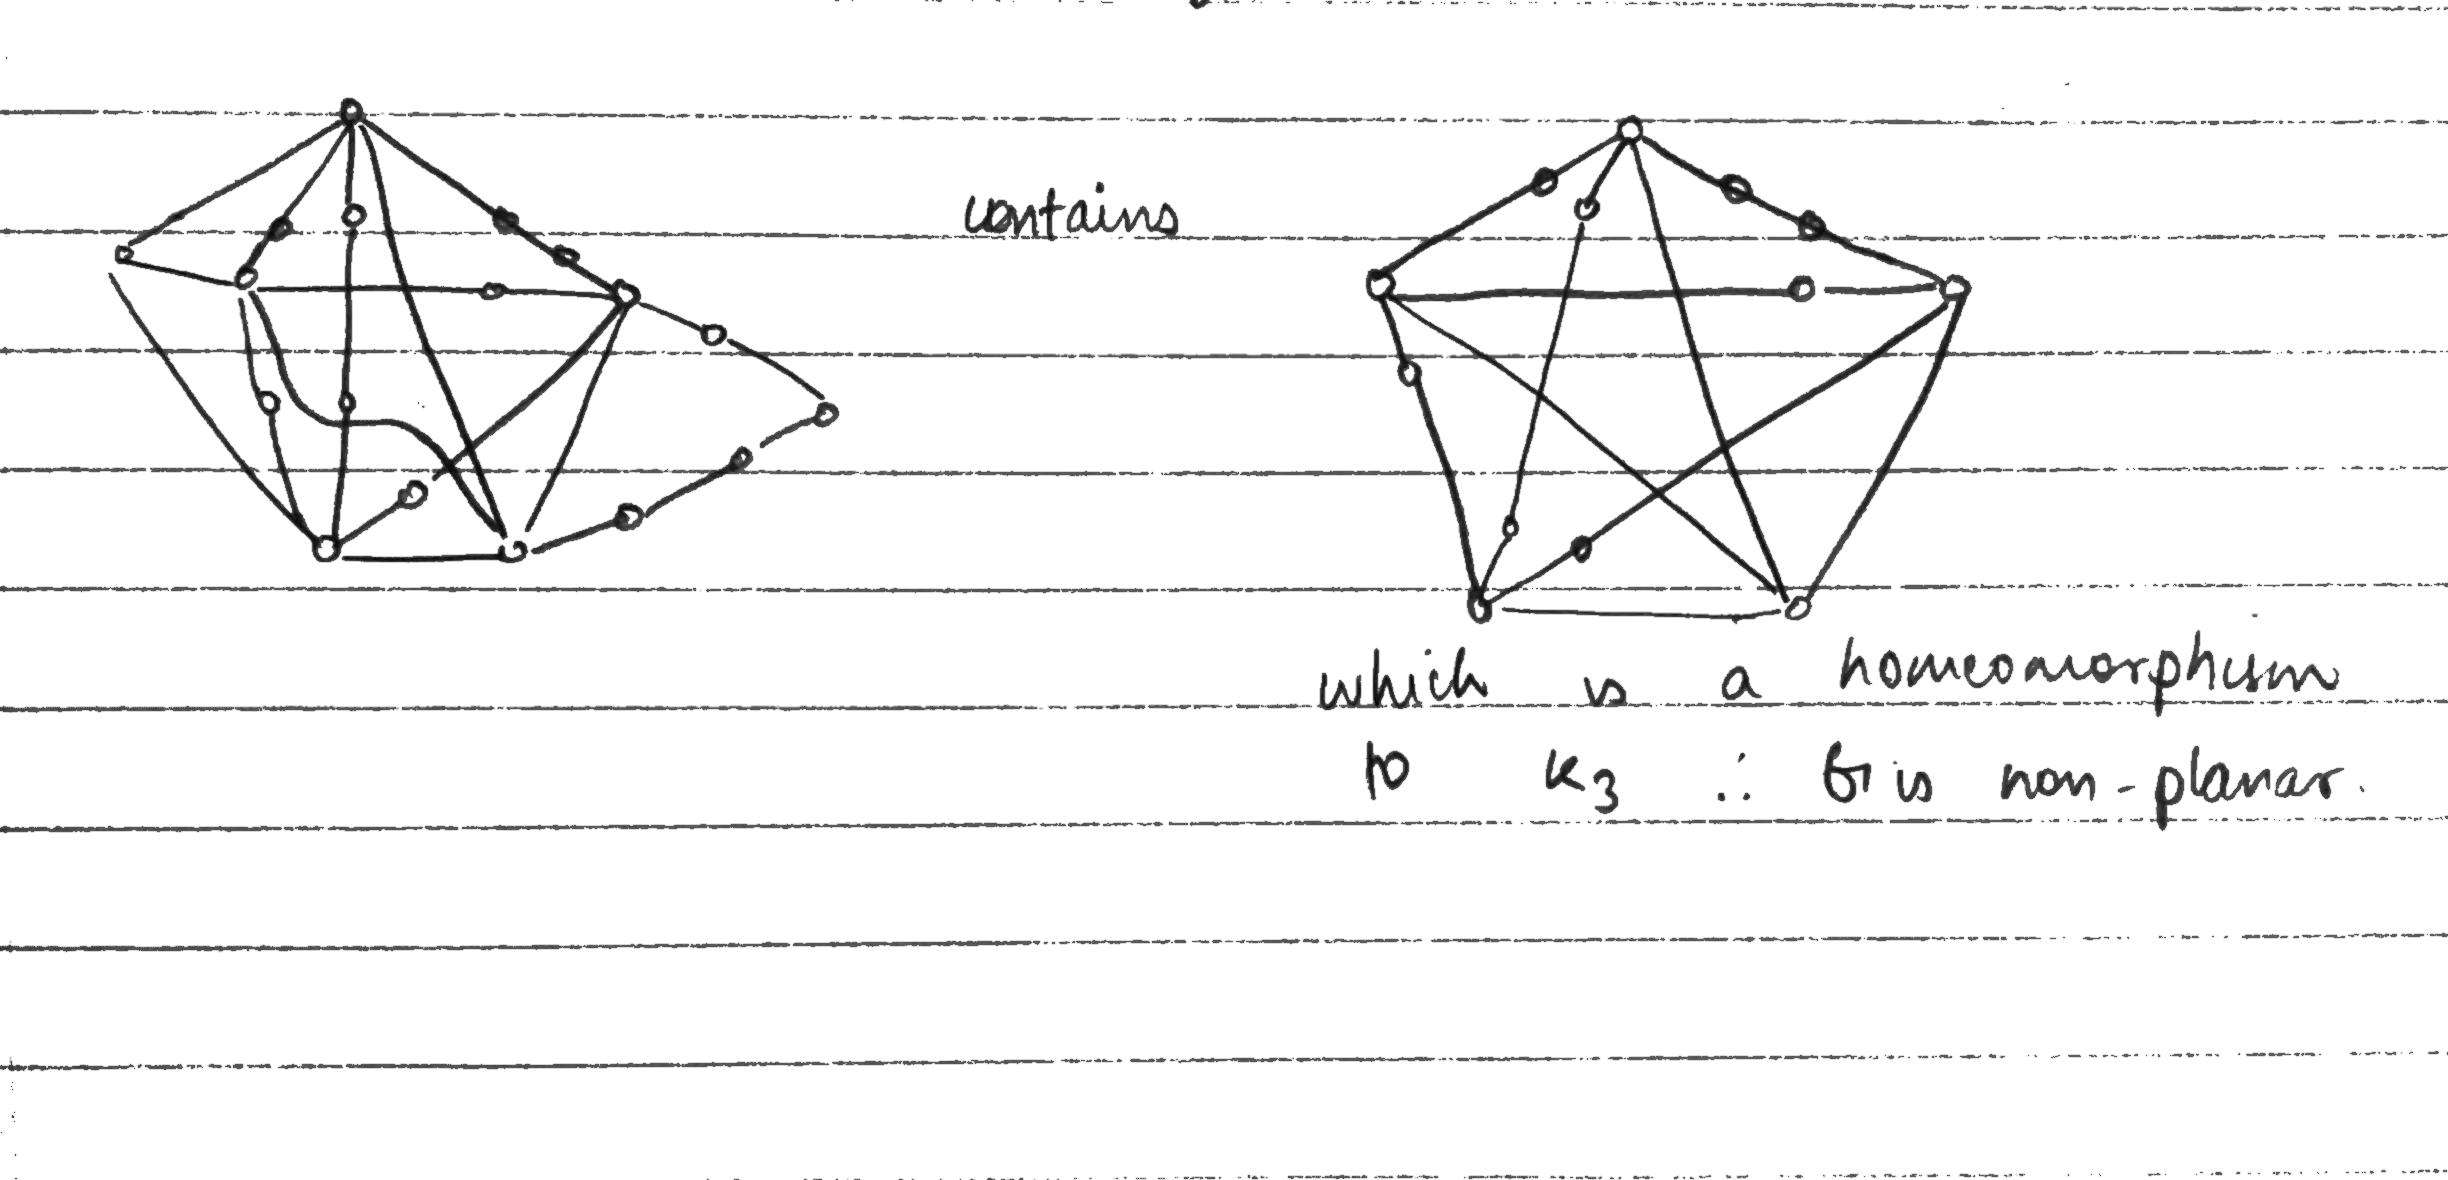
\includegraphics[scale=0.2]{petersan}
	\end{center}



	an alternate characterization of non-planar graphs can be obtained using the notion of contradictions.
\end{example}



\begin{definition}
	Let $G$ and $H$ be graphs. $G$ is said to be \underline{contractible to $H$} if $H$ can be obtained from $G$ by successivily contracting a finite number of edges.
\end{definition}


\begin{theorem}{6}
	A graph $G$ is planar if and only if it contains no subgraph which is contractible to $K_{5}$ or $K_{3,3}$.
\end{theorem}


\begin{example}

	Peterson graph is contractible to $K_{5}$.
	\begin{center}
		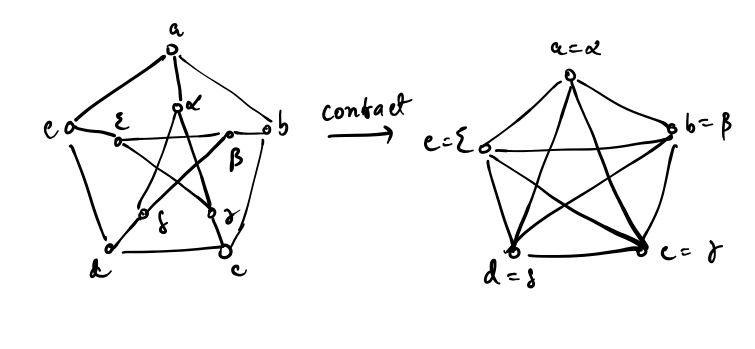
\includegraphics[scale=0.5]{petersansan}
	\end{center}


	Thus peterson is non-planar.
\end{example}


We have observed that $K_{5}$ and $K_{3,3}$ are non-planar. What happens if we consult other surface?

\begin{example}
	Torous (Donut)
	\begin{center}
		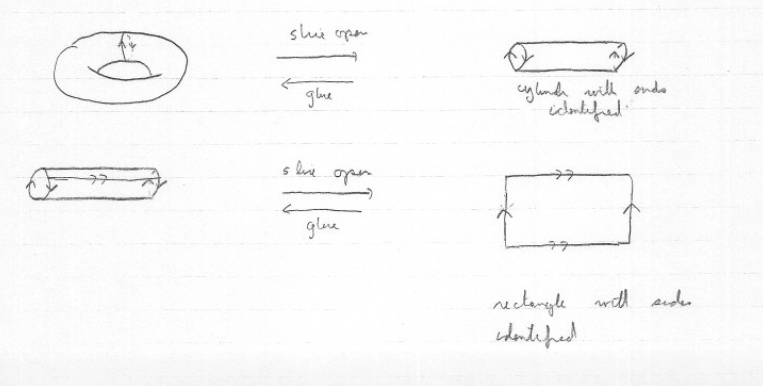
\includegraphics[scale=0.5]{toros}
	\end{center}
\end{example}


\begin{definition}
	A non-planar graph $G$ is said to be \underline{toroidal} if it can be drawn on the torus so as no two edges cross.
\end{definition}


\begin{example}
	\begin{enumerate}
		\item $K_{5}$ is torodial

		      \begin{center}
			      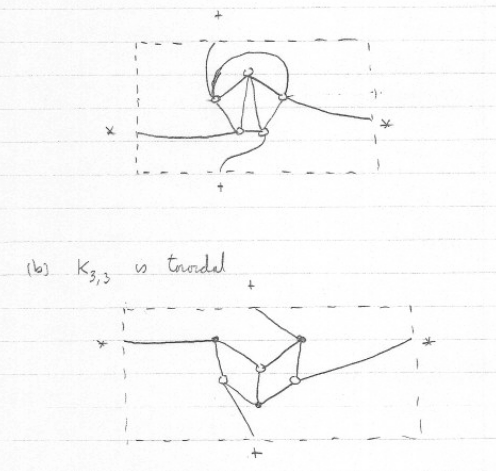
\includegraphics[scale=0.5]{torodial}
		      \end{center}

		\item $K_{3,3}$ is torodial

	\end{enumerate}

\end{example}


\textbf{Question:} Is there analogous of Euler's Formula for the toros?


\begin{theorem}{7}
	Let $G$ be a simple connected torodial graph of order $n$, size $m$ and $f$ faces, Then
	\[n - m + f = 0\]

	Furthermore,
	\[m \le \frac{gr(G)}{gr(G) - 2} n\]
\end{theorem}



\begin{definition}
	A graph $G$ is said to have genus $g$ if $G$ can be drawn on a surface of genus $g$ with no edges crossing, but no drawing on a surface of genus $g-1$ exists. (i.e planar = genus 0, torodial = genus 1)
\end{definition}



\begin{theorem}{8}
	Let $G$ be a connected graph of genus $g$, order $n$, size $m$, and face $f$. Then
	\[n - m + f = 2-2g\]
	Furthermore, if $G$ is simple of finite girth then
	\[m \le \frac{gr(G)}{gr(G) - 2} (n + 2g - 2)\]
\end{theorem}

\begin{corollary}
	Let $G$ be a connected simple graph of genus $g$, order $n\ge 3$ and size $m$ then,
	\[m \le 3(n+2g-2) \]
	\[m \le 2(n+2g-2) \text{ if no triangle present }\]
\end{corollary}


\begin{corollary}
	Let $G$ be a connected simple graph of order $n\ge 4$ and size $m$. Then the genus $g$ satisfies

	\[g \ge \lceil \frac{m-3n}{6} + 1 \rceil\]

	$\lceil x \rceil =$ least integer greater than or equal to $x$
\end{corollary}

\begin{remark}
	Let $G$ be a graph. The \underline{crossing number} $cr(G)$ is the minimum \# of crossing that can occur when $G$ is drawn in the plane.
\end{remark}

\begin{example}
	\textbf{graph here}
\end{example}


\begin{theorem}{9}
	The genus of the graph $G$ is $\le cr(G)$
\end{theorem}


\textbf{Dual Graphs}

\begin{definition}
	Let $G$ be a planar graph. The \underline{geometric dual} $G^{*}$ of $G$ is the graph constructed as follows:
	\begin{enumerate}
		\item denote each face of $G$, choose a point $v^{*}$. The $v^{*}$ forms the vertex set $V(G^{*})$
		\item For each edge $e$ of $G$, join the vertices $v^{*}$ and $w^{*}$ in the adjacent face by a curve $e^{*}$ that crosses $e$ and no other edge of $G$. The collection of $e^{*}$ froms the edge set $E(G^{*})$
	\end{enumerate}

\end{definition}

\begin{example}

	Platonic Graphs
	\begin{center}
		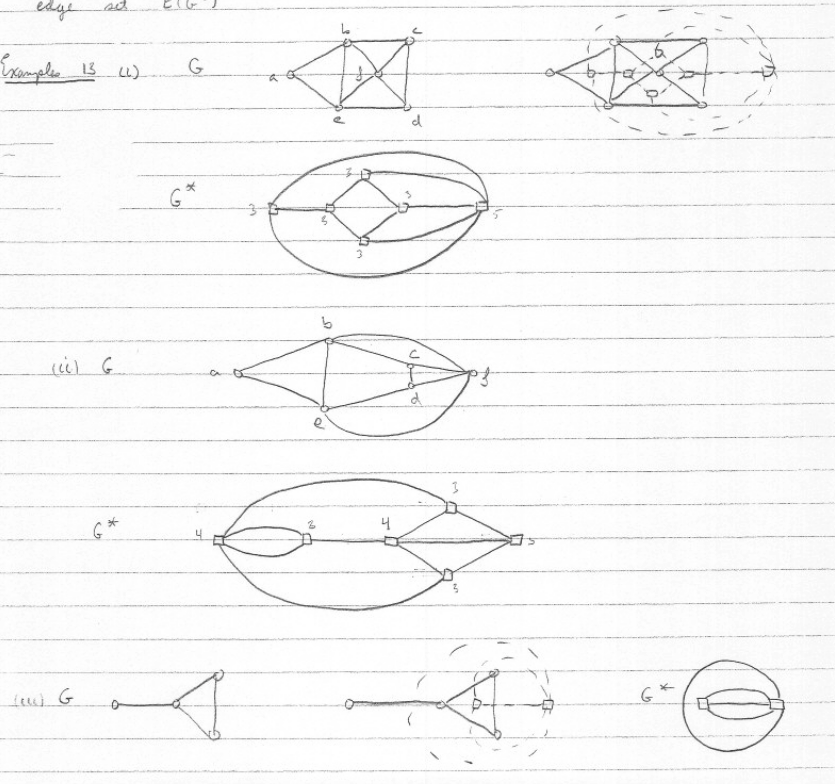
\includegraphics[scale=0.5]{dualgraph}
	\end{center}


	\begin{table}[H]
		\begin{center}
			\begin{tabular}{lll}
				\uline{\textbf{Graphs}} & \uline{\textbf{Geometric Dual}} &           \\
				tetrahedron             & tetrahedron                     & self-dual \\
				cube                    & octahedron                      &           \\
				octahedron              & cube                            &           \\
				dodecahedron            & icosahedron                     &           \\
				icosahedron             & dodecahedron                    &
			\end{tabular}
		\end{center}
	\end{table}

\end{example}



\begin{remark}
	\begin{enumerate}
		\item The contrustion of $G^{*}$ depends on the plane drawing of $G$. For example, the grphs $G$ in example 13 (i) and (ii) are isomorphic, bnut their geometric duals are not.  One has vertex of degree 5 but the other has no such vertex.
		\item $G^{*}$ is planar and connected.
	\end{enumerate}
\end{remark}


\begin{lemma}
	Let $G$ be a connected planar graph of order $n$, size $m$, and face $f$. If $G^{*}$ is a geometric dual then the nodes $n^{*}$ size $m^{*}$ and number of faces $f^{*}$ satisfies
	\[n^{*} = f, m^{*} = m, f^{*} =f\]
\end{lemma}


\begin{theorem}{10}
	Let $G$ be a connected planar graph. Then $G^{**}$ is isomorphic to $G$.
\end{theorem}

\begin{theorem}{11}
	Let $G$ be a connected planar graph and $G^{*}$ a geometric dual of $G$, A subset of $E(G)$ forms a cycle of $G$ if and only if the corresponding subset of $E(G^{*})$ is a cutset of $G^{*}$.
\end{theorem}

\begin{remark}
	If $e$ is an edge of $G$ then there is a unique edge $e^{*}$ of $G^{*}$ which crosses a
\end{remark}


% TODO



\begin{corollary}
	Let $G$ be a connected planar graph. A set of edges of $G$ forms a cutset if and only if the corresponding edges of $G^{*}$ forms a cycle.
\end{corollary}

\begin{theorem}{12}
	Let $G$ be a connected planar graph $G$ is bipartite if and only if $G^{*}$ is eulerian.
\end{theorem}


\begin{theorem}{13}
	Let $G$ be a connected planar graph. If $G$ is 3-edge connected then $G^{*}$ is simple (of order $\ge 3$)
\end{theorem}

\begin{definition}
	Let $G$ be a graph. A graph $G^{*}$ is said to be an \underline{abstract dual} of $G$ if there exists a one-one correspondence between the edge of $G$ and the of $G^{*}$ with the property that

	a subset of $E(G)$ forms a cycle $\leftrightarrow$ correspong subset of $E(G^{*})$ forms a cutset
\end{definition}

\begin{example}
	If $G$ is plane then its geometric dual $G^{*}$ is an abstract dual (Theorem 11)
	\begin{center}
		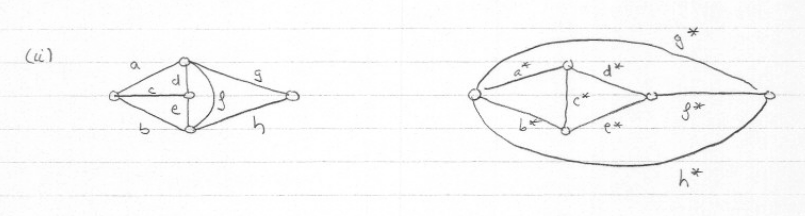
\includegraphics[scale=0.5]{dual2}
	\end{center}

\end{example}


\begin{theorem}{14}
	If $G^{*}$ is an abstract dual of $G$ then $G$ is an abstract dual of $G^{*}$.

	Abstract duals provide another characterization of planar graphs.
\end{theorem}

\begin{theorem}{15}
	A graph $G$ is planar if and only if $G$ has an abstract dual.
\end{theorem}


\end{document}
